\documentclass[12pt]{article}
\usepackage[margin=2cm]{geometry}
\usepackage{titling}
\usepackage[T1]{fontenc}
\usepackage[utf8]{inputenc}
\usepackage{tabularx}
\usepackage{graphicx}
\usepackage{amsmath}
\usepackage{amssymb}
\usepackage{algorithm}
\usepackage[noend]{algpseudocode}

\pretitle{\begin{center}\Huge\bfseries}
\posttitle{\par\end{center}\vskip 0.5em}
\preauthor{\begin{center}\Large}
\postauthor{\end{center}}
\predate{\par\large\centering}
\postdate{\par}

\title{Algorytmy Metaheurystyczne - lab 1}
\author{Jakub Musiał 268442}
\date{Listopad 2023}

\begin{document}

\maketitle

\section*{Cykl komiwojażera - algorytm Local Search}

\subsection*{Opis problemu}
    Wyznaczyć cykl komiwojażera dla grafu pełnego używając algorytmu \textit{Local Search} ze zdefiniowanym
    otoczeniem $N(\pi) = \{\pi' \in S(P) : (\exists \text{ } i \ne j)(\pi' = invert(\pi, i, j))\}$,
    gdzie $P$ - wejściowy zbiór punktów.
    \newline
    Otoczenie $invert$ zastosowane w algorytmie przeszukiwania lokalnego na grafach euklidesowych
    gwarantuje "rozplątanie" przecinających się krawędzi. Wynika to z faktu, że dystans euklidesowy
    jest metryką, zatem z nierówności trójkąta dla tej metryki możemy zauważyć, że dla pewnych punktów
    $p_1, p_2, p_3, p_4$ możemy zbudować 2 nieizomorficzne cykle:
    \begin{figure}[h]
        \centering
        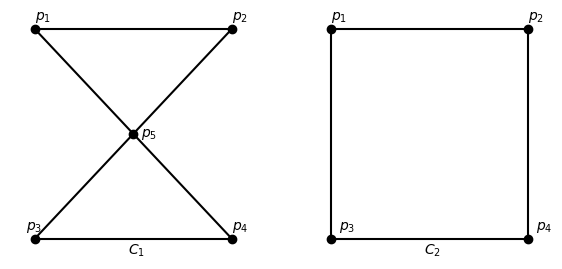
\includegraphics[scale=0.6]{img/euclidean_cycles.png}
        \label{fig:euclidean_cycles}
    \end{figure}
    \newline
    W cyklu $C_1$ punkt $p_5$ jest punktem przecięcia odcinków $\overline{p_1p_4}$ oraz $\overline{p_2p_3}$.
    Wiedząc zatem, że $d(p, q)$ jest metryką euklidesową mamy:
    $$ d(p_1,p_3) \leq d(p_1,p_5) + d(p_3,p_5) $$
    $$ d(p_2,p_4) \leq d(p_2,p_5) + d(p_4,p_5) $$
    Stąd zatem możemy pokazać, że $w(C_2) \leq w(C_1)$:
    $$w(C_1) = d(p_1,p_2) + d(p_2,p_3) + d(p_3,p_4) + d(p_4,p_1) =$$
    $$= d(p_1,p_2) + d(p_2,p_5) + d(p_5,p_3) + d(p_3,p_4) + d(p_4,p_5) + d(p_5,p_1) \geq$$
    $$\geq d(p_1,p_2) + d(p_2,p_4) + d(p_4,p_3) + d(p_3,p_1) = w(C_2) \text{   } \Box$$

    \newpage

    \noindent Dla odległości $d'(p, q) = round(d(p, q))$ (zaokrąglenie do najbliższej liczby
    całkowitej), jak w badanych grafach natomiast nie mamy już takiej gwarancji. Jako przykład
    weźmy pod uwagę wyżej opisane cykle i przyjmijmy, że
    $p_1 = (1,2) \land p_2 = (2,2) \land p_3 = (1,1) \land p_4 = (2,1)$.
    \newline
    Wtedy możemy zauważyć, że:
    $$w(C_1) = d'(p_1,p_2) + d'(p_2,p_3) + d'(p_3,p_4) + d'(p_4,p_1) = 1 + 1 + 1 + 1 = 4$$
    $$w(C_2) = d'(p_1,p_2) + d'(p_2,p_4) + d'(p_4,p_3) + d'(p_3,p_1) = 1 + 1 + 1 + 1 = 4$$
    Zatem $w(C_1) = w(C_2)$.
    \newline

\subsection*{Rozwiązanie}

    Poniżej przedstawiona jest procedura wyznaczania cyklu komiwojażera oraz
    alagorytm \textit{Local Search} dla zadanego problemu.

    \begin{algorithm}
    \caption{Wyznaczanie cyklu komiwojażera}\label{alg:tsp_cycle}
    \begin{algorithmic}[1]
        \Require $P$
        \State $G \gets graph(P)$
        \State $MST_G \gets prim\_mst(G)$
        \State $\pi_0 \gets dfs\_order(MST_G)$
        \State $\pi \gets local\_seach(\pi_0)$
    \end{algorithmic}
    \end{algorithm}

    \begin{algorithm}[h!]
    \caption{Wyznaczanie cyklu komiwojażera}\label{alg:local_search}
    \begin{algorithmic}[1]
        \Procedure{$local\_search$}{$\pi_0$}
            \State $\pi \gets \pi_0$
            \State $w_\pi \gets weight(\pi)$
            \State $l_\pi \gets length(\pi)$
            \State
            \While{$true$}
                \State $w_b \gets w_\pi$
                \State $(i_b, j_b) \gets (0, 0)$
                \For{$i \gets 0$ to $l_\pi$}
                    \For{$j \gets i + 1$ to $l_\pi$}
                        \State $w_{invert} \gets invert\_weight(\pi, i, j)$
                        \If{$w_{invert} < w_b$}
                            \State $w_b \gets w_{invert}$
                            \State $(i_b, j_b) \gets (i, j)$
                        \EndIf
                    \EndFor
                \EndFor
                \State
                \If{$w_b \geq w_\pi$}
                    \Return $\pi$
                \EndIf
                \State
                \State $\pi \gets invert(\pi, i_b, j_b)$
                \State $w_\pi \gets w_b$
            \EndWhile
        \EndProcedure
    \end{algorithmic}
    \end{algorithm}

\newpage

\subsection*{Wyniki}
    Poniższe tabele oraz wykresy przedstawiają wyniki otrzymane dla poszczególnych zadań.

    \subsubsection*{Zadanie 1 - losowy wierzchołek startowy w MST}

        \begin{table}[h!]
        \centering
        \begin{tabularx}{0.745\textwidth}{| c | c | c | c | c |}
            \hline
            Dane wejściowe & $w(MST)$ & $avg(w(TSC))$ & $w(TSC_{min})$ & $avg(n_{impr})$ \\
            \hline
            xqf131 & $474$ & $605$ & $587$ & $24$ \\
            xqg237 & $897$ & $1104$ & $1081$ & $50$ \\
            pma343 & $1179$ & $1483$ & $1470$ & $72$ \\
            pka379 & $1151$ & $1411$ & $1387$ & $85$ \\
            bcl380 & $1444$ & $1755$ & $1727$ & $72$ \\
            pbl395 & $1124$ & $1363$ & $1345$ & $81$ \\
            pbk411 & $1180$ & $1438$ & $1424$ & $85$ \\
            pbn423 & $1201$ & $1479$ & $1450$ & $92$ \\
            pbm436 & $1269$ & $1558$ & $1540$ & $98$ \\
            xql662 & $2240$ & $2683$ & $2642$ & $127$ \\
            xit1083 & $3253$ & $3822$ & $3773$ & $223$ \\
            icw1483 & $4015$ & $4828$ & $4759$ & $309$ \\
            djc1785 & $5541$ & $6605$ & $6568$ & $376$ \\
            dcb2086 & $5950$ & $7137$ & $7085$ & $410$ \\
            pds2566 & $6956$ & $8260$ & $8166$ & $466$ \\
            \hline
        \end{tabularx}
        \label{table:ex1}
        \end{table}

    \newpage

    \subsubsection*{Zadanie 2 - losowa permutacja startowa}

        \begin{table}[h!]
        \centering
        \begin{tabularx}{0.745\textwidth}{| c | c | c | c | c |}
            \hline
            Dane wejściowe & $w(MST)$ & $avg(w(TSC))$ & $w(TSC_{min})$ & $avg(n_{impr})$ \\
            \hline
            xqf131  & $474$  & $611$  & $579$  & $133$  \\
            xqg237  & $897$  & $1118$ & $1066$ & $260$  \\
            pma343  & $1179$ & $1485$ & $1427$ & $403$  \\
            pka379  & $1151$ & $1446$ & $1403$ & $448$  \\
            bcl380  & $1444$ & $1817$ & $1729$ & $447$  \\
            pbl395  & $1124$ & $1427$ & $1355$ & $458$  \\
            pbk411  & $1180$ & $1489$ & $1417$ & $483$  \\
            pbn423  & $1201$ & $1523$ & $1455$ & $496$  \\
            pbm436  & $1269$ & $1609$ & $1534$ & $512$  \\
            xql662  & $2240$ & $2812$ & $2706$ & $811$  \\
            xit1083 & $3253$ & $4021$ & $3906$ & $1384$ \\
            icw1483 & $4015$ & $4986$ & $4855$ & $1930$ \\
            djc1785 & $5541$ & $6878$ & $6733$ & $2344$ \\
            dcb2086 & $5950$ & $7463$ & $7289$ & $2798$ \\
            pds2566 & $6956$ & $8695$ & $8547$ & $3483$ \\
            \hline
        \end{tabularx}
        \label{table:ex2}
        \end{table}

    \subsubsection*{Zadanie 3 - losowe inwersje}

        \begin{table}[h!]
        \centering
        \begin{tabularx}{0.745\textwidth}{| c | c | c | c | c |}
            \hline
            Dane wejściowe & $w(MST)$ & $avg(w(TSC))$ & $w(TSC_{min})$ & $avg(n_{impr})$ \\
            \hline
            xqf131 & $474$ & $720$ & $669$ & $1$ \\
            xqg237 & $897$ & $1434$ & $1330$ & $2$ \\
            pma343 & $1179$ & $1884$ & $1806$ & $2$ \\
            pka379 & $1151$ & $1834$ & $1767$ & $3$ \\
            bcl380 & $1444$ & $2317$ & $2188$ & $1$ \\
            pbl395 & $1124$ & $1845$ & $1713$ & $2$ \\
            pbk411 & $1180$ & $1971$ & $1832$ & $2$ \\
            pbn423 & $1201$ & $1977$ & $1909$ & $2$ \\
            pbm436 & $1269$ & $2066$ & $1939$ & $2$ \\
            xql662 & $2240$ & $3637$ & $3461$ & $2$ \\
            xit1083 & $3253$ & $5182$ & $5044$ & $2$ \\
            icw1483 & $4015$ & $6647$ & $6381$ & $2$ \\
            djc1785 & $5541$ & $8867$ & $8633$ & $2$ \\
            dcb2086 & $5950$ & $9796$ & $9438$ & $2$ \\
            pds2566 & $6956$ & $11363$ & $10989$ & $3$ \\
            \hline
        \end{tabularx}
        \label{table:ex3}
        \end{table}

    \newpage

    \newgeometry{top=1.3cm,bottom=1.3cm,left=2cm,right=2cm}

    \subsubsection*{Badane wartości w zależności od liczby wierzchołków grafu}

        \begin{figure}[h]
            \centering
            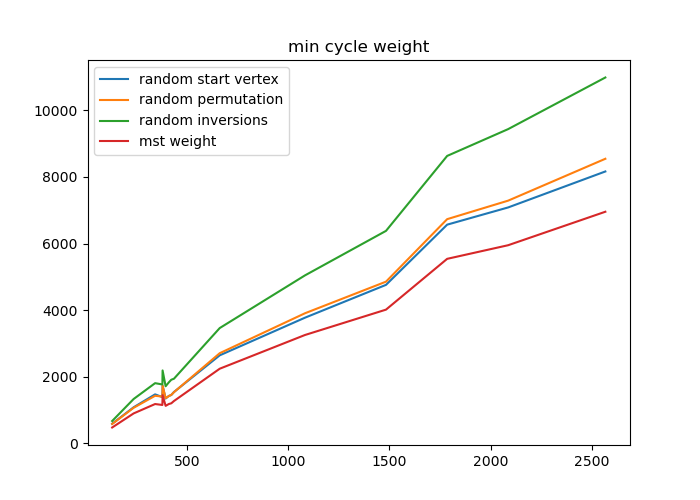
\includegraphics[width=0.75\linewidth]{img/min_cycle_weight.png}
            \label{fig:min_cycle_weight}
            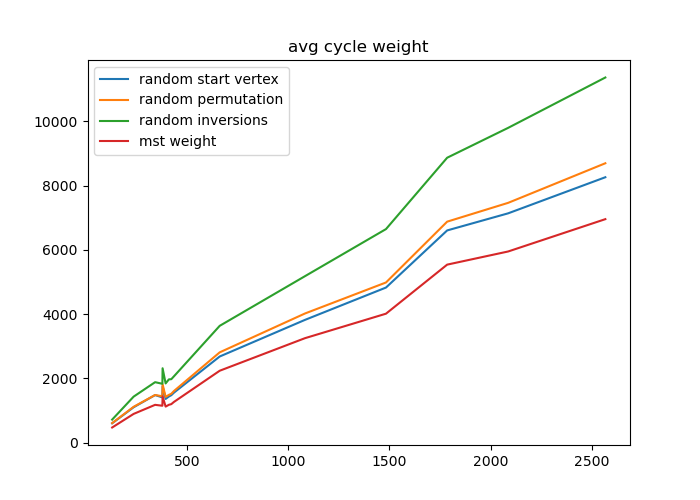
\includegraphics[width=0.75\linewidth]{img/avg_cycle_weight.png}
            \label{fig:avg_cycle_weight}
        \end{figure}
        \newpage
        \begin{figure}[h]
            \centering
            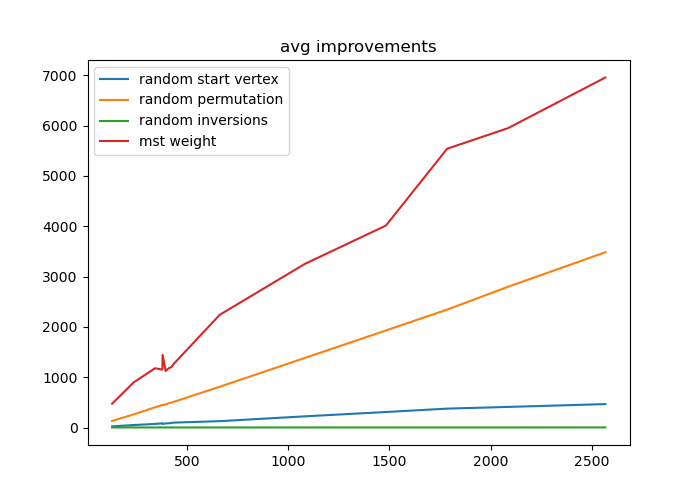
\includegraphics[width=0.75\linewidth]{img/avg_improvements.png}
            \label{fig:avg_improvements}
        \end{figure}

    \subsubsection*{Wizualizacja cykli komiwojażera wyznaczonych w zadaniu 1}

        \begin{figure}[h]
            \centering
            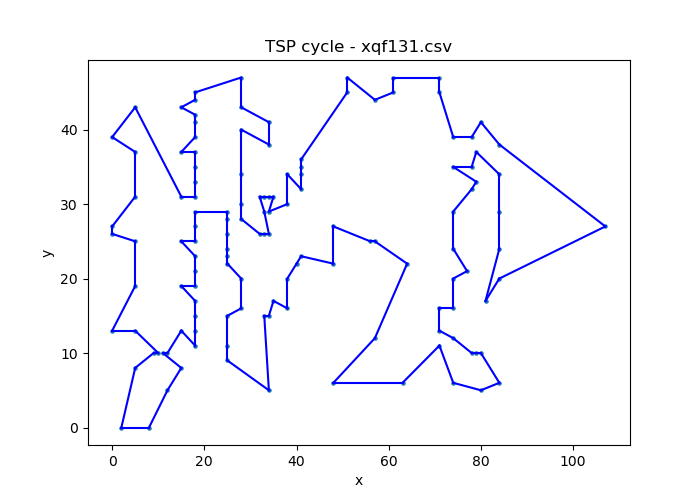
\includegraphics[width=0.74\linewidth]{img/xqf131.png}
            \label{fig:xqf131}
        \end{figure}

        \newpage

        \begin{figure}[h]
            \centering
            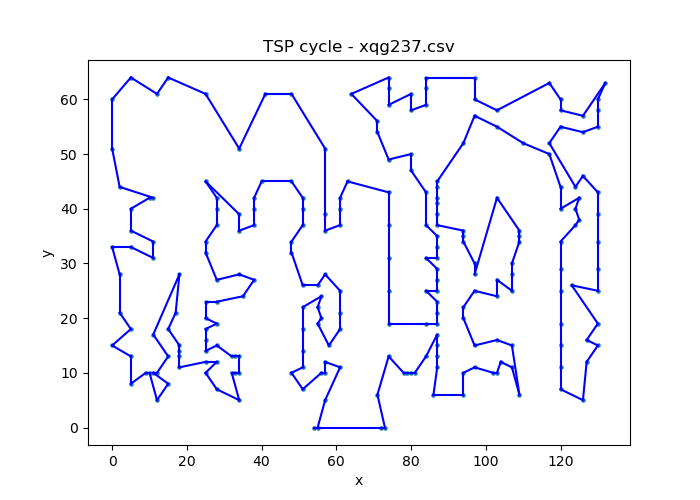
\includegraphics[width=0.8\linewidth]{img/xqg237.png}
            \label{fig:xqg237}
            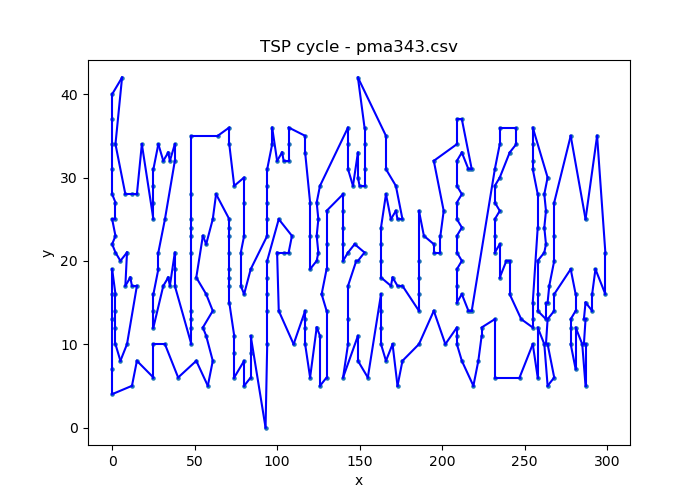
\includegraphics[width=0.8\linewidth]{img/pma343.png}
            \label{fig:pma343}
        \end{figure}

        \newpage

        \begin{figure}[h]
            \centering
            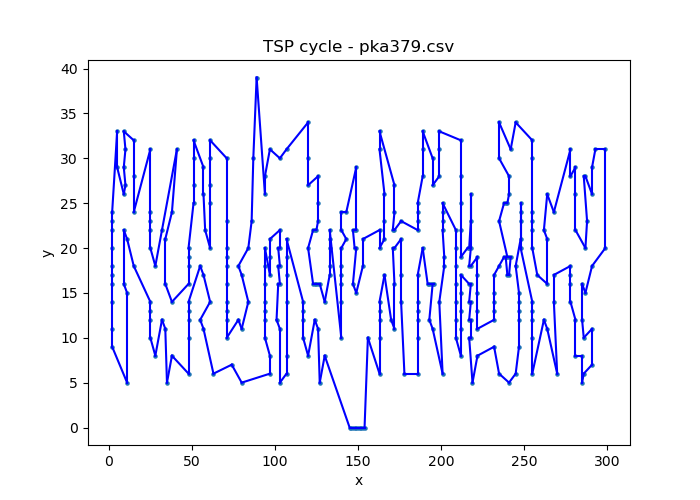
\includegraphics[width=0.8\linewidth]{img/pka379.png}
            \label{fig:pka379}
            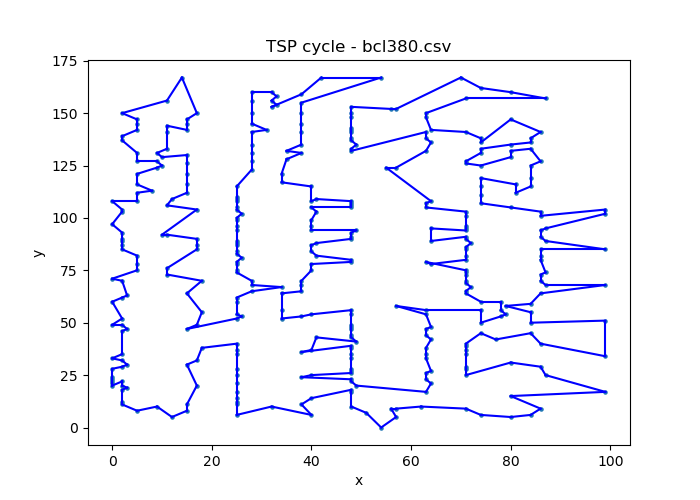
\includegraphics[width=0.8\linewidth]{img/bcl380.png}
            \label{fig:bcl380}
        \end{figure}

        \newpage

        \begin{figure}[h]
            \centering
            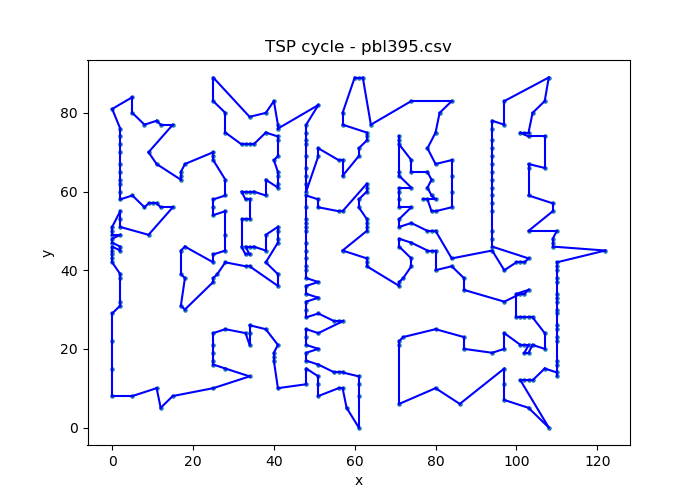
\includegraphics[width=0.8\linewidth]{img/pbl395.png}
            \label{fig:pbl395}
            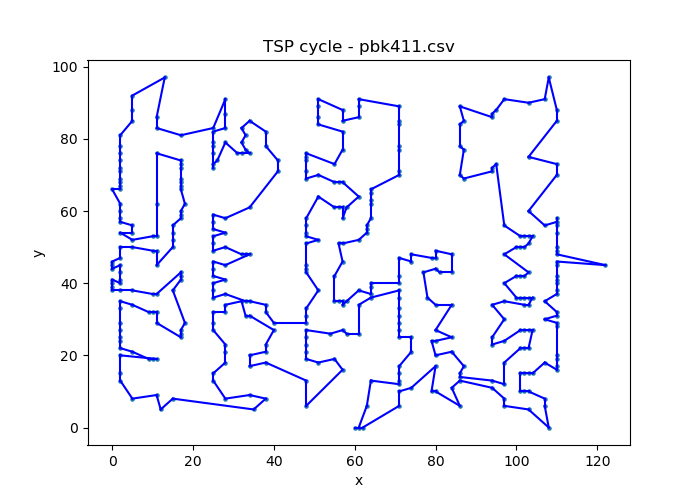
\includegraphics[width=0.8\linewidth]{img/pbk411.png}
            \label{fig:pbk411}
        \end{figure}

        \newpage

        \begin{figure}[h]
            \centering
            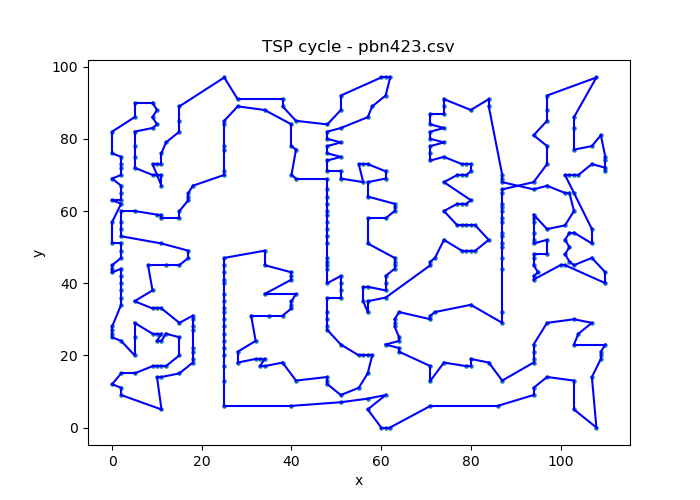
\includegraphics[width=0.8\linewidth]{img/pbn423.png}
            \label{fig:pbn423}
            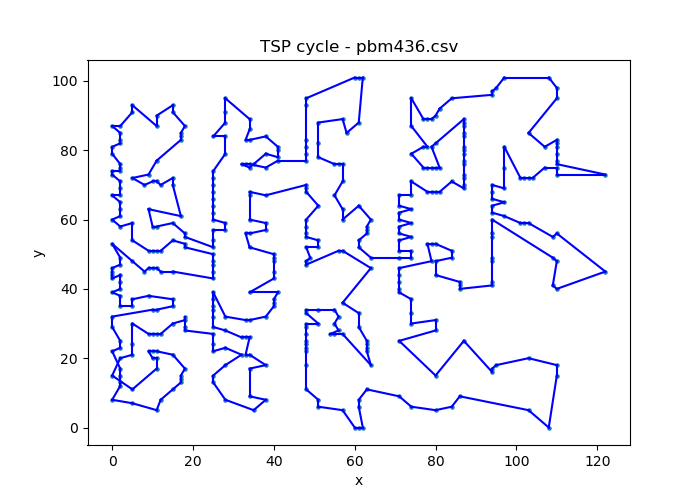
\includegraphics[width=0.8\linewidth]{img/pbm436.png}
            \label{fig:pbm436}
        \end{figure}

        \newpage

        \begin{figure}[h]
            \centering
            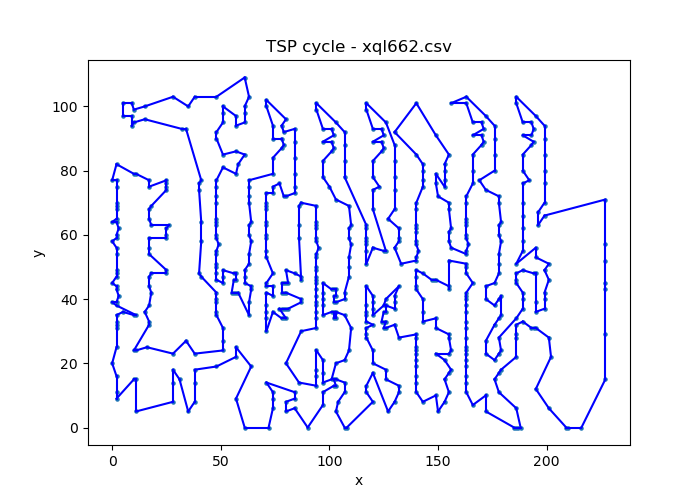
\includegraphics[width=0.8\linewidth]{img/xql662.png}
            \label{fig:xql662}
            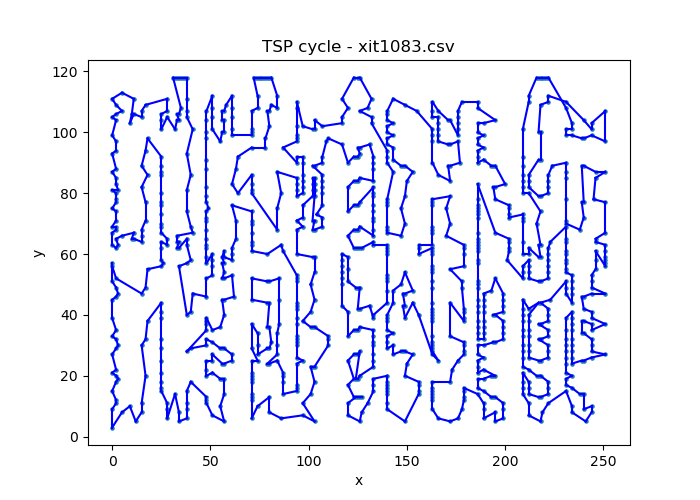
\includegraphics[width=0.8\linewidth]{img/xit1083.png}
            \label{fig:xit1083}
        \end{figure}

        \newpage

        \begin{figure}[h]
            \centering
            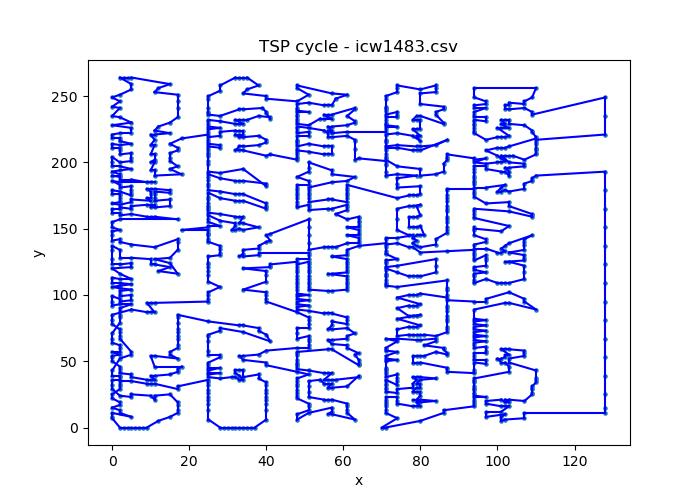
\includegraphics[width=0.8\linewidth]{img/icw1483.png}
            \label{fig:icw1483}
            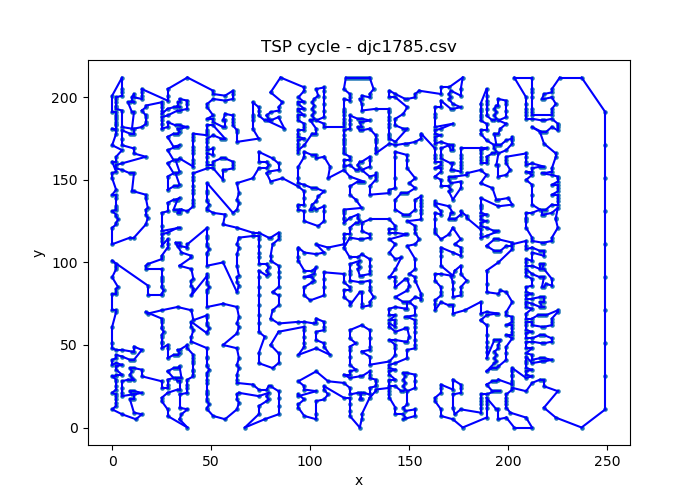
\includegraphics[width=0.8\linewidth]{img/djc1785.png}
            \label{fig:djc1785}
        \end{figure}

        \newpage

        \begin{figure}[h]
            \centering
            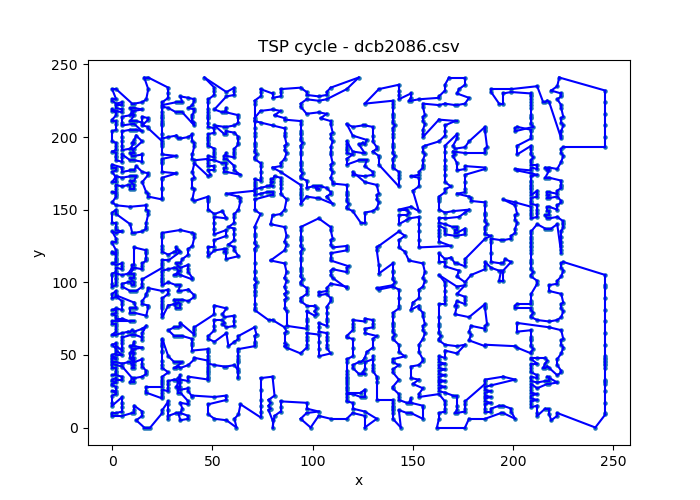
\includegraphics[width=0.8\linewidth]{img/dcb2086.png}
            \label{fig:dcb2086}
            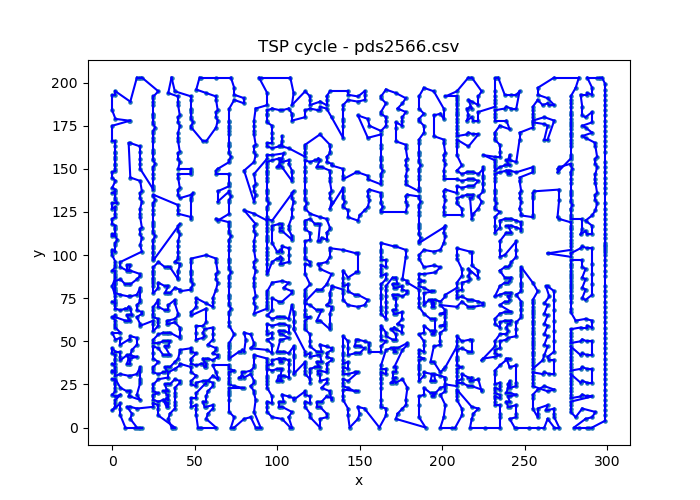
\includegraphics[width=0.8\linewidth]{img/pds2566.png}
            \label{fig:pds2566}
        \end{figure}

\newpage

\end{document}
